\begin{frame}{Τρωτά σημεία μεθόδων ευθυγράμμισης}

  \vspace{0.2cm}
  \noindent\makebox[0.65\linewidth][c]{%
  \begin{minipage}{0.5\linewidth}

    \begin{minipage}{0.3\linewidth}
      \begin{figure}
        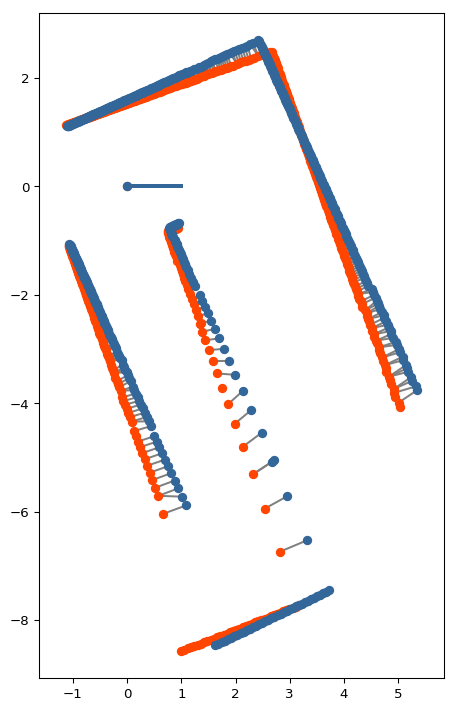
\includegraphics[scale=0.2]{./figures/slides/ch4/correspondence_is_the_culprit/pic0.png}
        \caption{\scriptsize Α}
      \end{figure}
    \end{minipage}
    \hfill
    \begin{minipage}{0.7\linewidth}
      \begin{figure}
        \animategraphics[scale=0.3,autoplay,loop]{2}{./figures/slides/ch4/correspondence_is_the_culprit/plicp/frame_}{00}{25}
        \caption{\scriptsize Β}
      \end{figure}
    \end{minipage}
  \end{minipage}
  }
  \noindent\makebox[0.3\linewidth][c]{%
  \begin{minipage}{0.3\linewidth}\scriptsize
    Α: ICP επί της αρχής (σημείο προς σημείο)\\

    Β: plicp: σημείο προς ευθύγραμμο τμήμα. Πηγή: Andrea Censi, \url{https://censi.science/research/robot-perception/plicp/}\\

    Γ: (a) Κατανομή προς κατανομή, (b) Σημείο προς κατανομή, (c) Κατανομή προς κατανομές. \\Πηγή: \textit{Voxelized GICP for Fast and Accurate 3D Point Cloud Registration}, ICRA 2021
  \end{minipage}
  }
  \noindent\makebox[0.65\linewidth][c]{%
  \begin{minipage}{\linewidth}
    \begin{figure}
      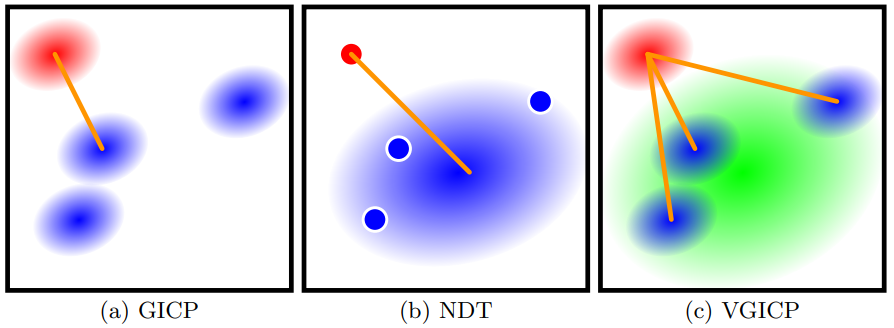
\includegraphics[scale=0.2]{./figures/slides/ch4/correspondence_is_the_culprit/gicp.png}
        \caption{\scriptsize Γ}
    \end{figure}
  \end{minipage}
  }


\end{frame}
